%
% hardware.tex
%
% Copyright (C) 2020 by SpaceLab.
%
% PC-104 Adapter Documentation
%
% This work is licensed under the Creative Commons Attribution-ShareAlike 4.0
% International License. To view a copy of this license,
% visit http://creativecommons.org/licenses/by-sa/4.0/.
%

%
% \brief Hardware overview chapter.
%
% \author Gabriel Mariano Marcelino <gabriel.mm8@gmail.com>
%
% \institution Universidade Federal de Santa Catarina (UFSC)
%
% \version 0.2.0
%
% \date 2020/09/25
%

\chapter{Hardware Overview} \label{ch:hardware}

\cite{picoblade}

\section{Top Board}

\begin{figure}[!htb]
    \begin{center}
        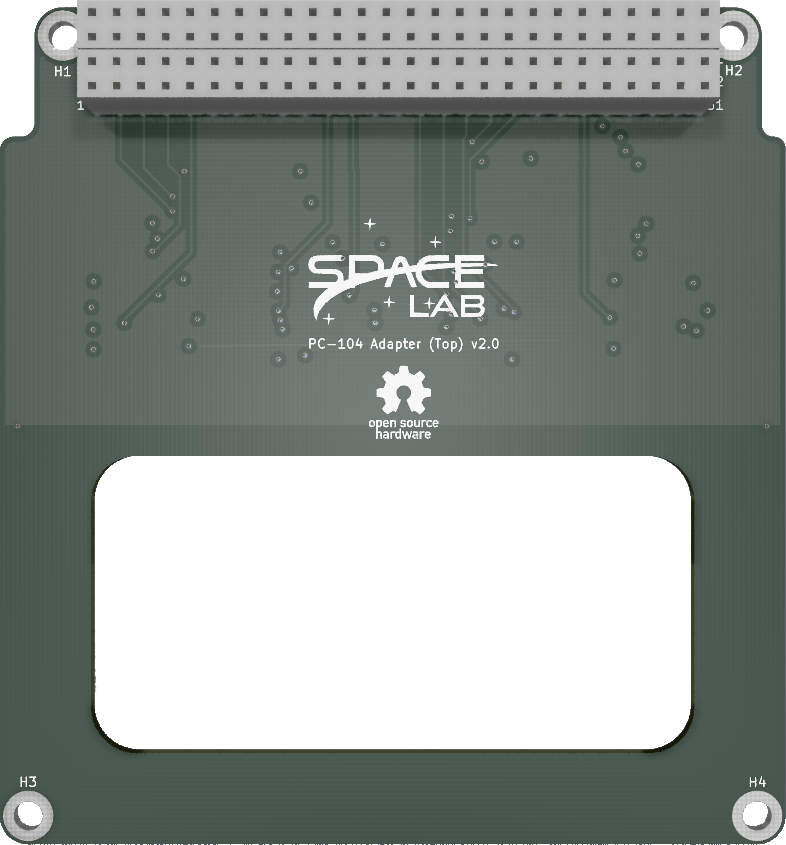
\includegraphics[width=8.636cm]{figures/pc104-adapter-top-top}
        \caption{Top view of the top board (real size).}
        \label{fig:top-board-top}
    \end{center}
\end{figure}

\begin{figure}[!htb]
    \begin{center}
        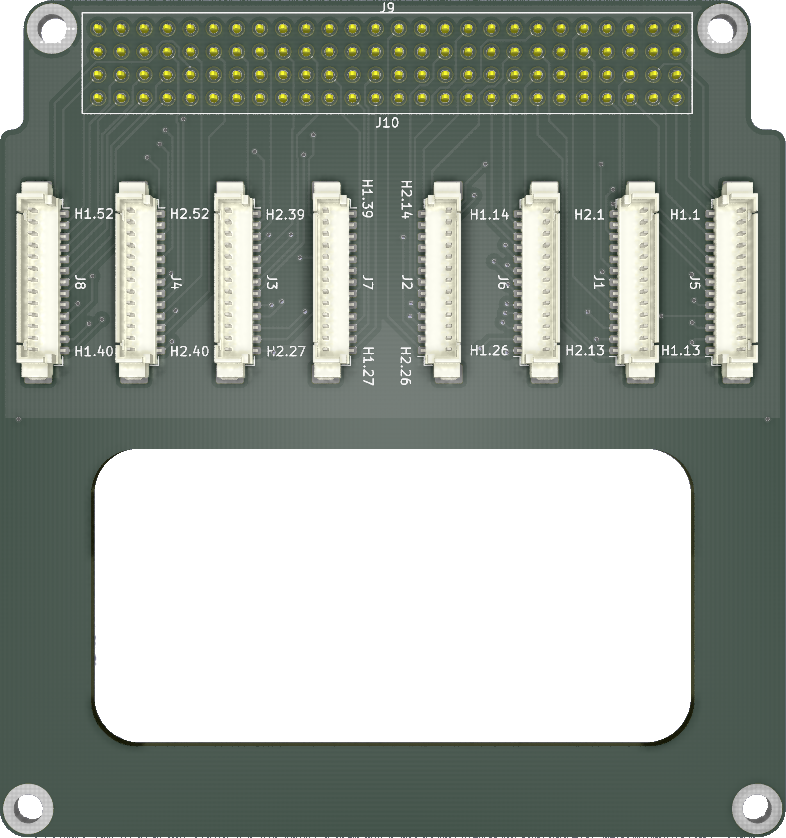
\includegraphics[width=8.636cm]{figures/pc104-adapter-top-bottom}
        \caption{Bottom view of the top board (real size).}
        \label{fig:top-board-bottom}
    \end{center}
\end{figure}

\section{Bottom Board}

\begin{figure}[!htb]
    \begin{center}
        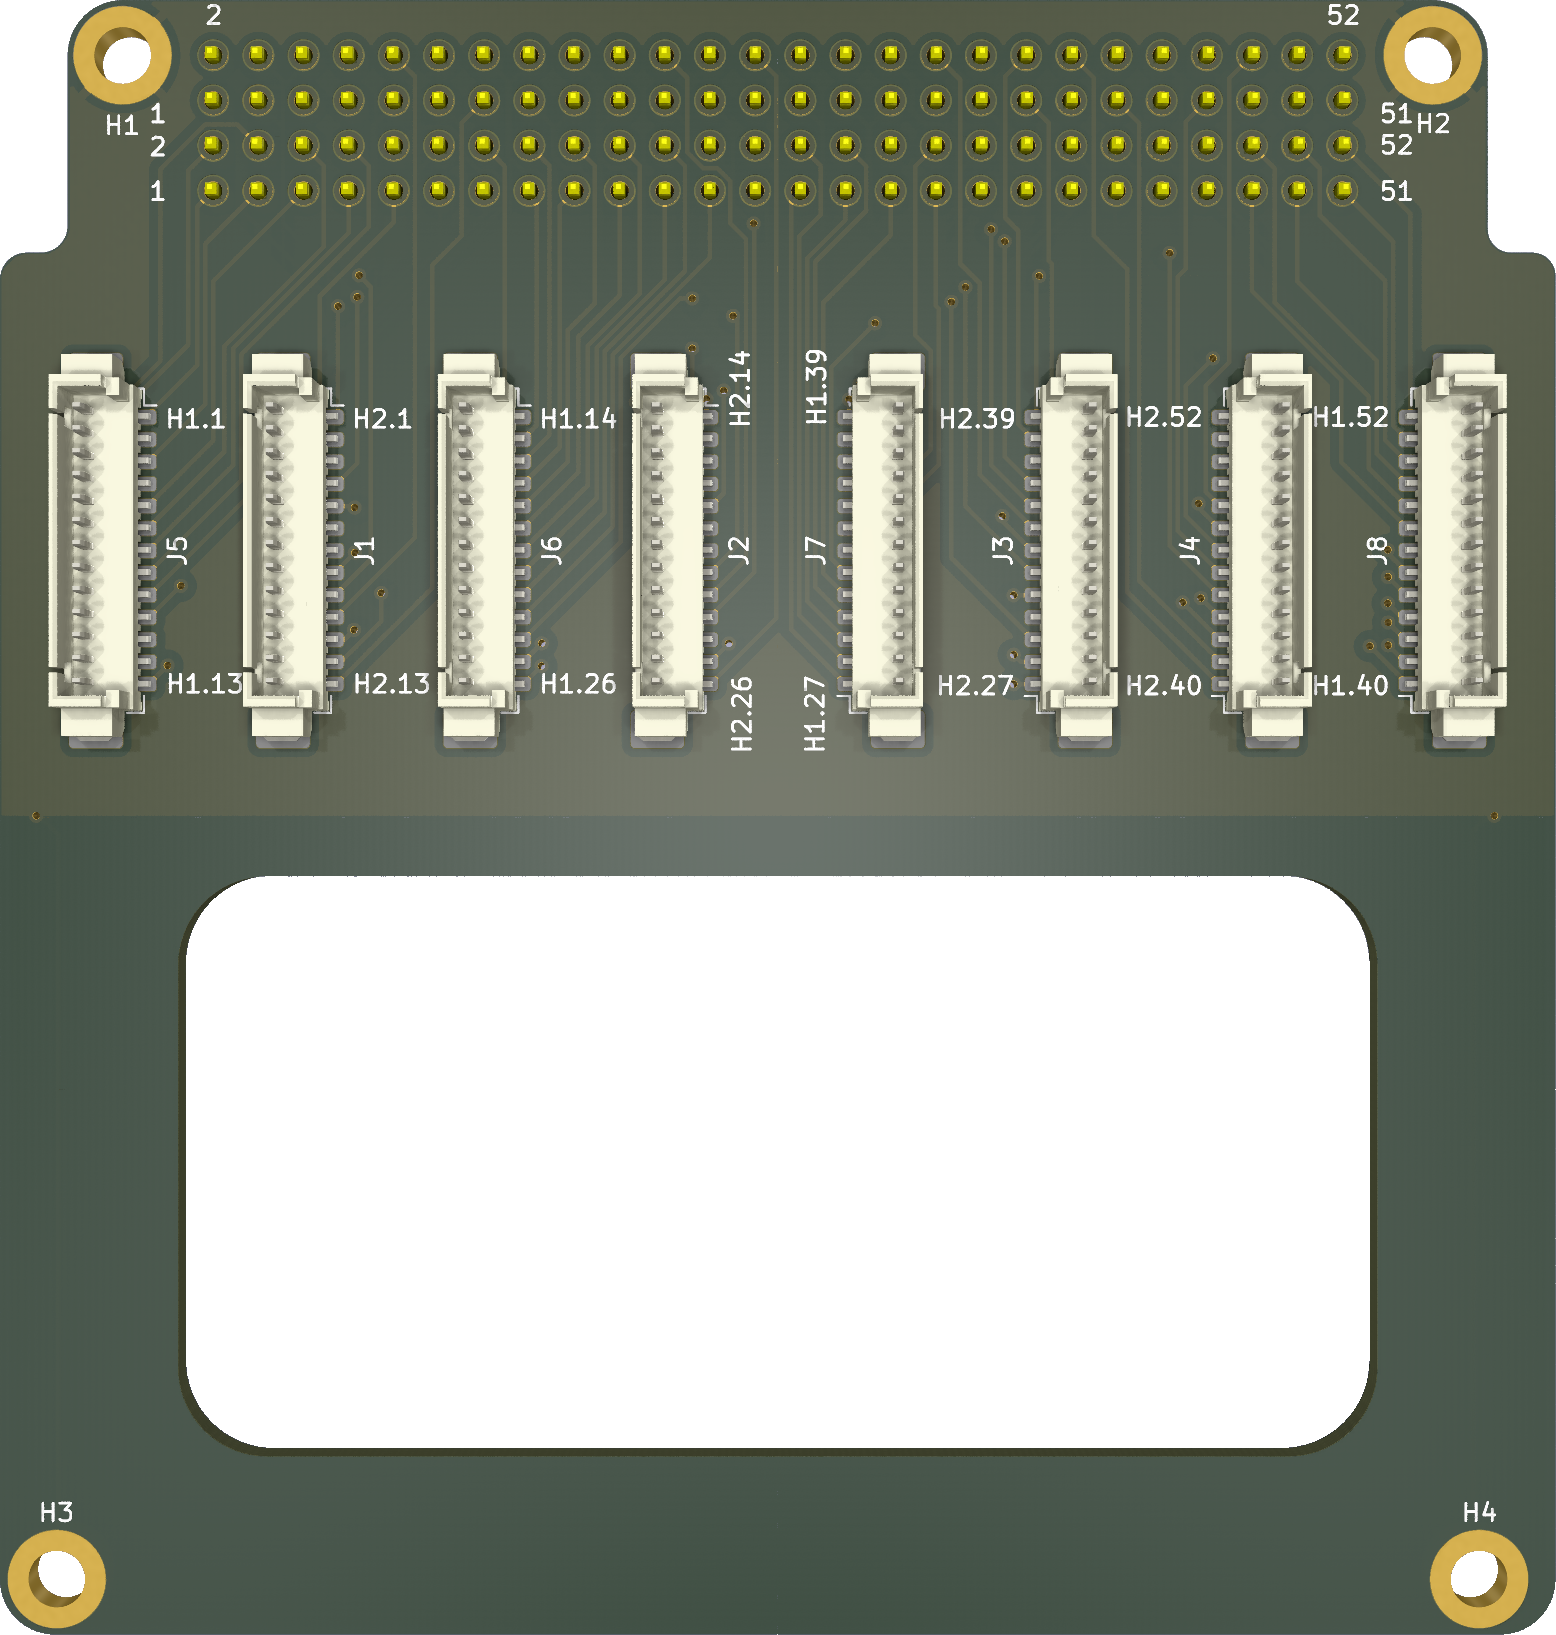
\includegraphics[width=8.626cm]{figures/pc104-adapter-bottom-top}
        \caption{Top view of the bottom board (real size).}
        \label{fig:bottom-board-top}
    \end{center}
\end{figure}

\begin{figure}[!htb]
    \begin{center}
        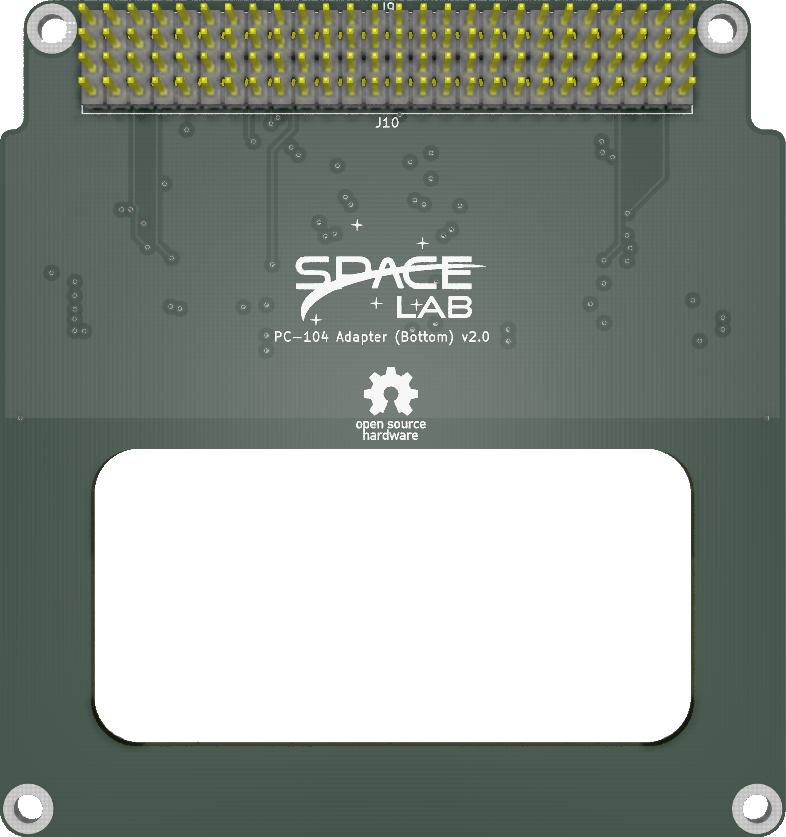
\includegraphics[width=8.626cm]{figures/pc104-adapter-bottom-bottom}
        \caption{Bottom view of the bottom board (real size).}
        \label{fig:bottom-board-bottom}
    \end{center}
\end{figure}

